\chapter{Statistical Analysis} \label{chapter:statistical-analysis}
Having prepared the bond data and matched it with the stocks, some statistical analysis can now be performed. In particular, we are interested in summary statistics of corporate bond returns, as well as in the analysis of the lead-lag relationship of corporate bond and stock returns. For this, the returns themselves need to be calculated from daily prices first. Additionally, as the matching has so far only been done for static data, it needs to be extended to historical return data as well. All in all, the following procedure for the statistical analysis arises: 
\begin{enumerate}
	\item calculate monthly bond returns
	\item match bond and equity returns
	\item calculate summary statistics
	\item analyze lead-lag relationship
\end{enumerate}

\section{Monthly Bond Returns}
In order to calculate the monthly bond returns, the following formula will be used: \\
$R_{n} = \dfrac{P_{n}}{P_{n-1}}$, \\ where $R_{n}$ stands for bond return for month $n$, and $P_{n}$ for the bond price on last day of month $n$. 
To implement the formula in Stata, in the time series bond data only the last price of each bond for each month needs to be kept. The rest of the data can be dropped, as it is not relevant for the current analysis. The pricing parameter which will be used to calculate the returns is \textit{MPD}. It represents the Datastream Selected Default Price, and is the most reliable price parameter in the extracted database. Other price parameters, such as e.g. \textit{CP} (Clean Price), have significantly more missing values and are thus less suited for the purpose. Having kept the last monthly prices, a variable group consisting of the variables \textit{dscd} and \textit{month} has to be generated (\textit{egen} \textit{group} command). This group can then be set as a Stata time-series (\textit{tsset}). Based on the time-series, the monthly return variable can be generated with the introduced formula. The Stata do file for the task can be found in. %TODO  ref do_generate_monthly_returns

\section{Matching Bond and Equity Returns}
To match the bond and equity returns with each other, we can make use of the matching that we accomplished in chapter \ref{chapter:matching}. For this, we load the corporate bond returns, which we just calculated, into Stata. These bond returns can then be merged with the existing matching over the $bond_dscd$ parameter, as shown in Fig. \ref{fig:matching-returns}. 
\begin{figure}[h]
	\centering
	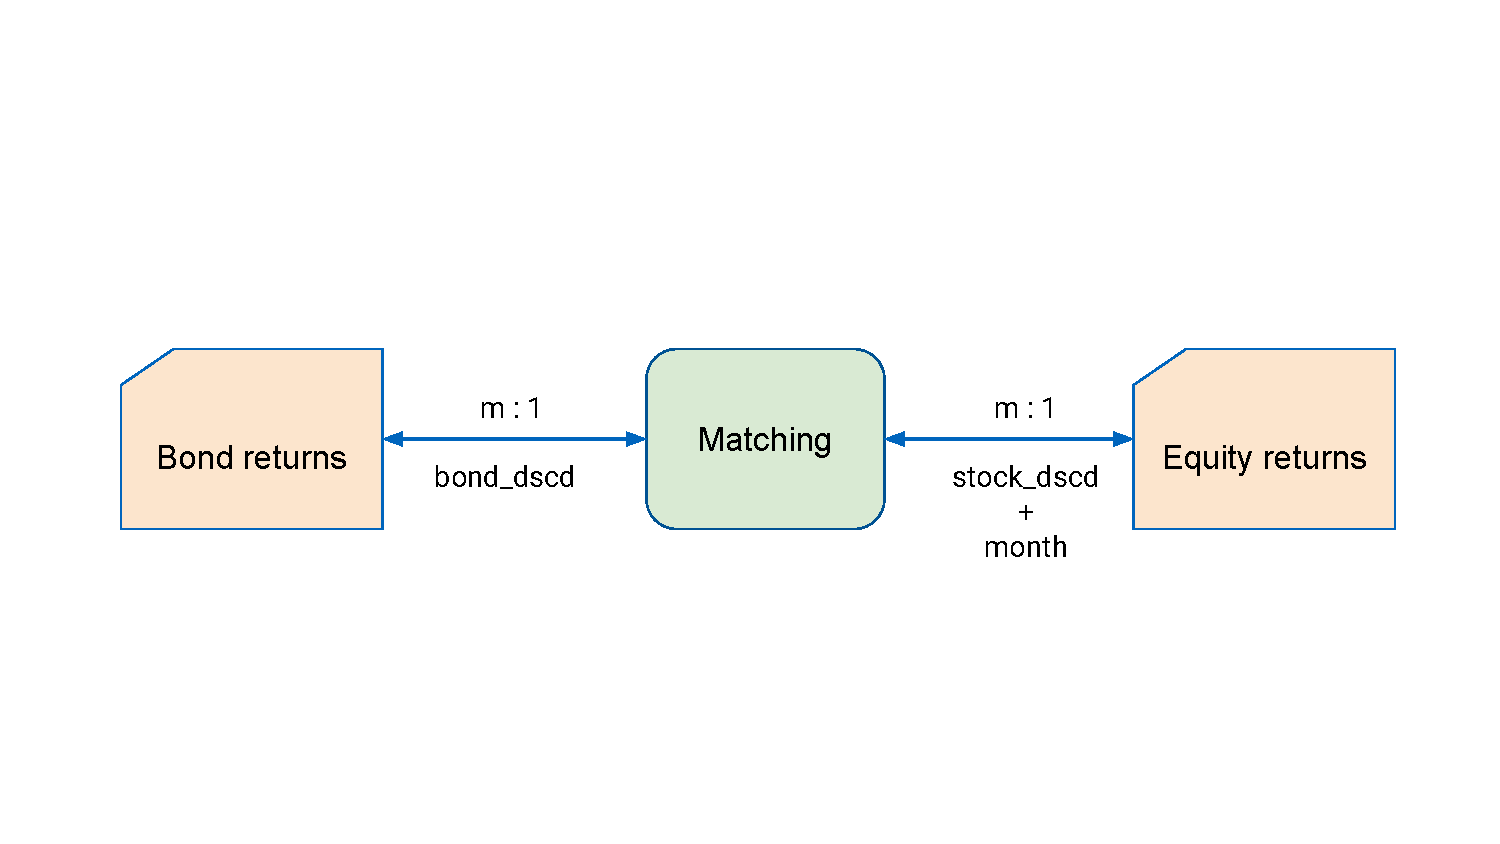
\includegraphics[trim={0 4.5cm 0 5cm},clip,width=1.0\linewidth]{figures/matching-returns.pdf}
	\caption{Matching of Bond and Equity Returns}
	\label{fig:matching-returns}
\end{figure}
After that, the resulting dataset has to be merged with the provided stock time series data, which also includes the required monthly stock returns. This merge should take place over the two parameters $stock\_dscd$ and $month$. This is because we want the bond and stock returns to be comparable for one and the same month later on. When executing the merges in Stata, keep in mind to make sure that the Datastream code parameter is named the same in the bond dataset and the matching (i.e. $bond\_dscd$), and similarly for the stocks and the matching (i.e. $stock\_dscd$). Otherwise, the matching will fail. The bonds-matching merge is performed on a M-to-1 relation, because multiple bonds can be mapped to the same equity over the issuing company. The merge with the equities is performed on a M-to-1 relation as well for the same reason. The resulting database builds the foundation for further statistical analysis. 

\section{Summary Statistics} \label{section:summary-statistics}
Stata offers very useful tools to determine the underlying distribution of the data, as well as to perform correlation and regression calculations. In order to obtain summary statistics separately for different bond groups, I split the bond returns dataset by geography and by credit rating. 

\begin{figure}[h]
	\centering
	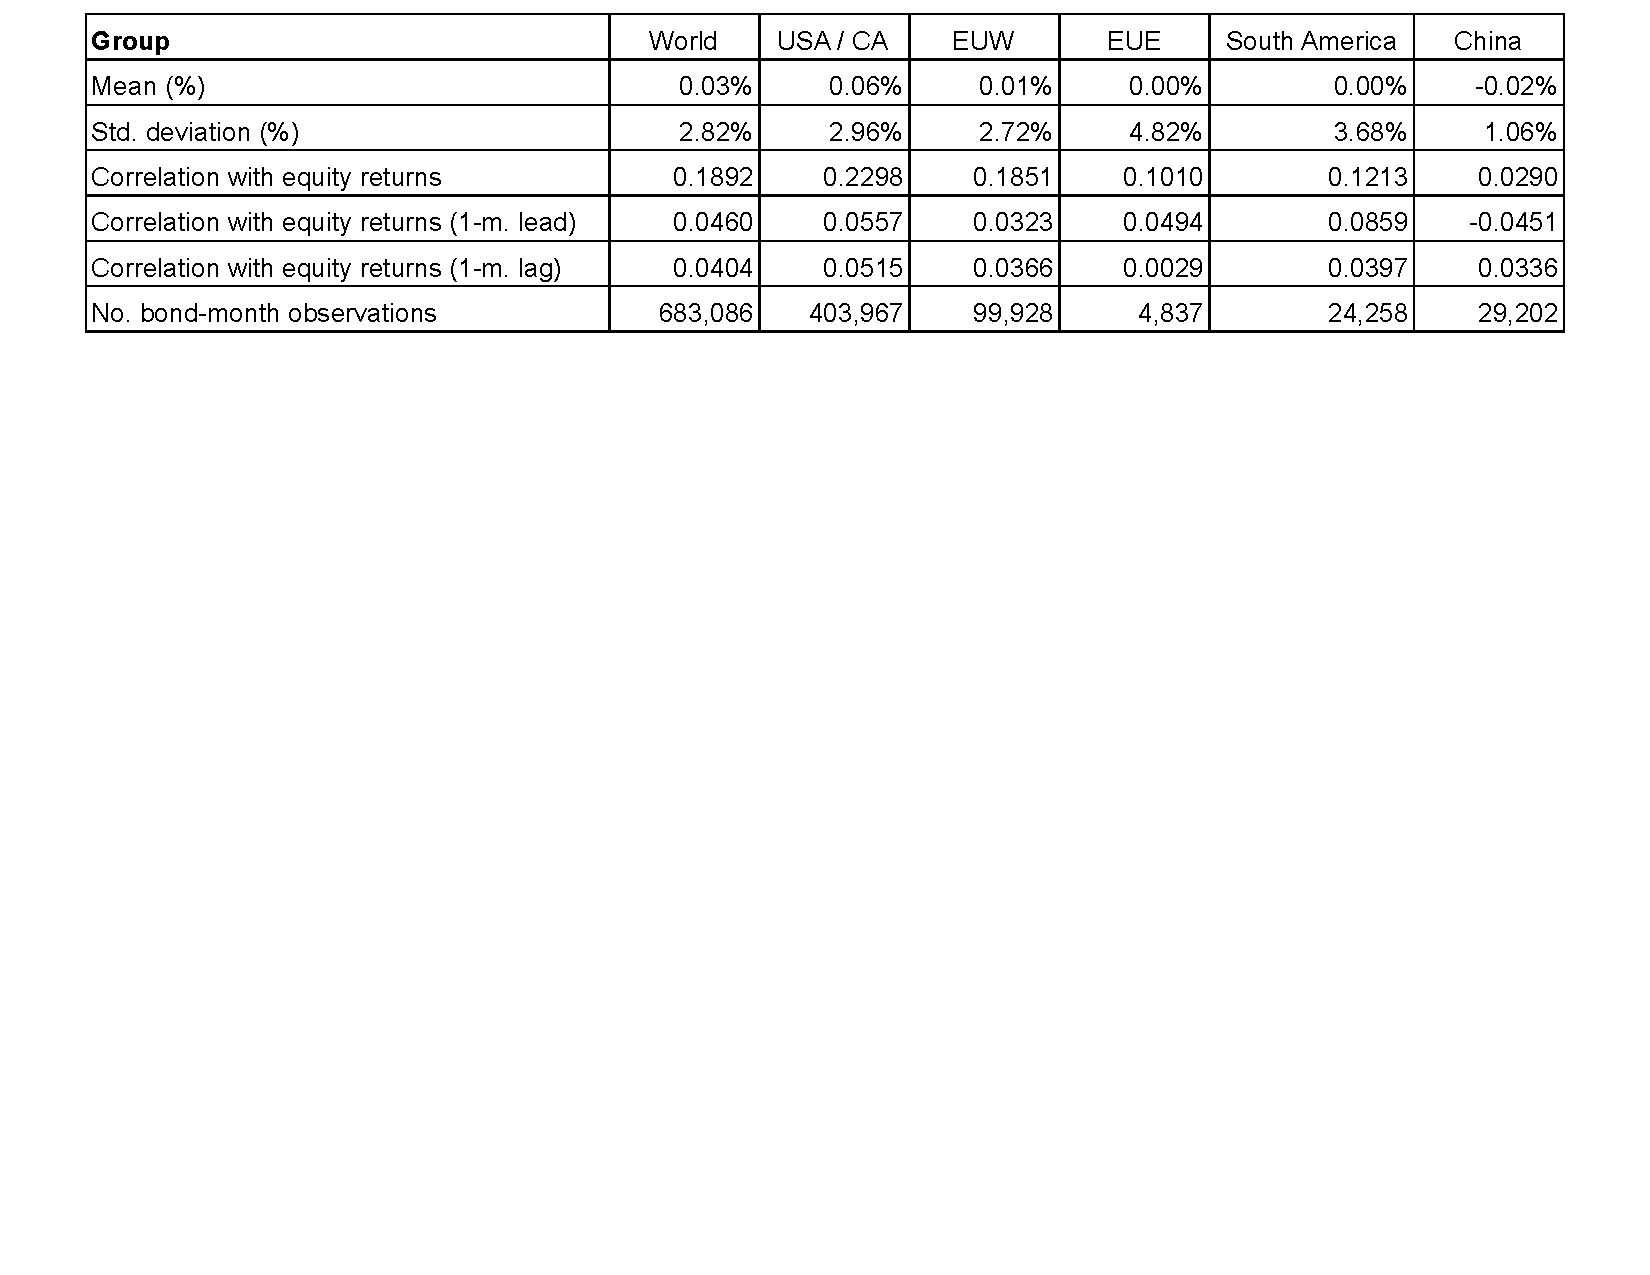
\includegraphics[trim={0 15.5cm 0 0},clip,width=1.0\linewidth]{figures/summary-stats-by-geo.pdf}
	\caption{Monthly Return Statistics by Bond Geography}
	\label{fig:summary-stats-by-geo}
\end{figure}

Fig. \ref{fig:summary-stats-by-geo} features monthly return statistics for:
\begin{itemize}
	\item The entire world
	\item North America region (NA), represented by USA and Canada
	\item Western Europe region (EUW), represented by Germany, France, UK, Italy, Ireland, Luxembourg, Netherlands, Spain, Portugal, Belgium, Austria, Switzerland, and Scandinavian countries
	\item Eastern Europe region (EUE), represented by Poland, Czech Republic, Bulgaria, Greece, Serbia, Croatia, Hungary, Montenegro, Ukraine, Turkey, and Georgia
	\item South America region, represented by Brazil, Argentina, Chile, Colombia, Uruguay, Paraguay, Panama, Peru, and Mexico (though NA)
	\item China 
\end{itemize}
Note that the list is neither regionally exhaustive, nor is it 100\% geographically accurate. Its sole purpose is to gain a general idea of the distribution of corporate bond returns for countries with a similar financial structure. 

Fig. \ref{fig:summary-stats-by-rating} features monthly return statistics for different credit ratings of corporate bonds. Please note that the number of bond-month observations for the single credit ratings does not sum up to to the number in the \textit{All} column. This is due to the procedure which was used to split the bonds up by their rating. To give an example, bonds listed in rating category \textit{BBB} are those bonds which have either a \textit{BBB} rating as given by the S\&P agency, or a \textit{Baa} rating as given by the Moody's agency. In some cases, it occurs that e.g. the Moody's rating is given as \textit{A}, and the S\&P rating as \textit{BBB}. In this case, the bond would be listed in both the \textit{A} and the \textit{BBB} categories, which results in intersections between the single categories. The procedure has been chosen this way to receive a larger amount of data for analysis, as e.g. entries for the Moody's rating alone were somewhat scarce. If needed, further analysis can be done based on ratings of a single agency only. 

\begin{figure}[h]
	\centering
	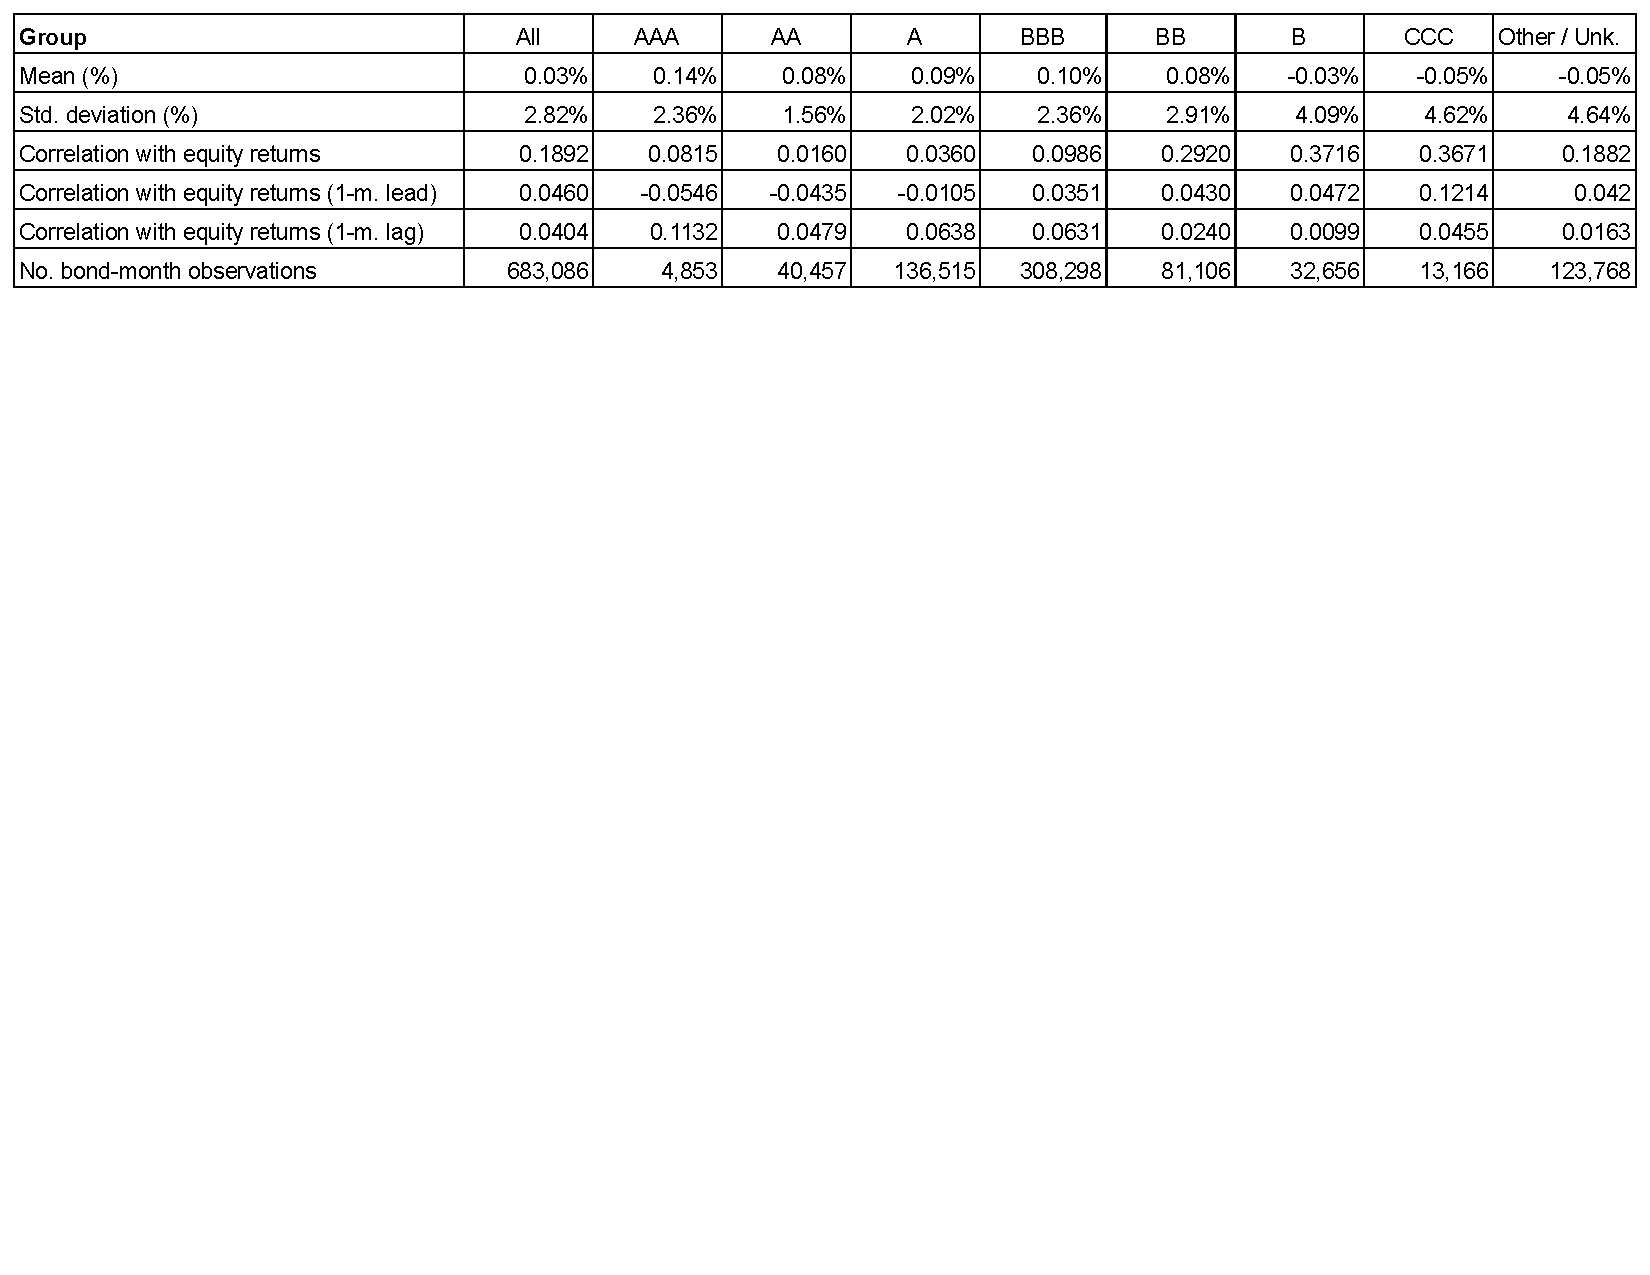
\includegraphics[trim={0 16cm 0 0},clip,width=1.0\linewidth]{figures/summary-stats-by-rating.pdf}
	\caption{Monthly Return Statistics by Bond Rating}
	\label{fig:summary-stats-by-rating}
\end{figure}

The distribution mean and standard deviation of the bond returns are largely in-line with my expectations. Bonds in regions with a majority of developed countries generally have a higher mean return and a lower standard deviation than bonds in regions with more developing countries. Similarly, investment grade bonds have higher mean return and lower volatility than non-investment grade bonds. 

The correlation with equity returns looks higher for developed regions, but at the same time lower for investment grade bonds. 
Additionally, the correlation of monthly bond returns with lagged stock returns strictly monotonically increases with falling credit rating. As such, the lowest bond-lead correlation can be seen for corporate bonds rated \textit{AAA}, while the highest correlation is listed for \textit{CCC} rated bonds. This already explains quite well why existing research on the topic of the lead-lag relation of corporate bonds and stocks mostly focuses on high yield bonds, as these have the highest lead correlation with stocks. The correlation results of stock returns with lagged bond returns are less conclusive, but tend to be higher for investment grade bonds. From a geographical point of view, there seems to be no significant insight for the lead and lag correlations with equity returns. 

\section{Lead-Lag Relationship} \label{section:lead-lag-relationship}
In order to estimate the existence of a potential lead or lag relationship between corporate bonds and stocks, multiple regression analyses have been run. In particular, the calculations were conducted for the following bond groups: 
\begin{itemize}
	\item all corporate bonds
	\item split by geographical region: North America, South America, Western Europe, Eastern Europe, and China
	\item split by bond credit rating: AAA, AA, A, BBB, BB, B, CCC, other
	\item split by aggregated bond credit rating: investment grade and non-investment grade bonds
	\item two rating-based approaches to high-yield bonds
\end{itemize}
All regression analyses have been run as a duo of: 
\begin{enumerate}
	\item regression with monthly bond returns as dependent variable and 1-month lagged stock returns as independent variable
	\item regression with monthly stock returns as dependent variable and 1-month lagged bond returns as independent variable
\end{enumerate}

For shortness, not all the regression results will be introduced here in detail. This section will mostly focus on high yield bonds, as these have shown the most likely lead correlation with equities in section \ref{section:summary-statistics}, and also because the leads and lags of high yield bonds have seen the highest attention in the existing literature on this subject so far. All the other regression results can be found either in the appendix to this work, or as part of the project files. %TODO ref regressions appendix

\begin{figure}[h]
	\centering
	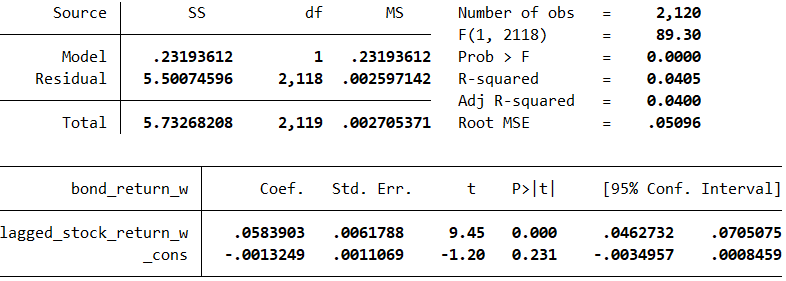
\includegraphics[trim={0 0 0 0},clip,width=1.0\linewidth]{figures/regression-results/regression-high-yield-ccc-d-moodies-bonds-as-dependent.PNG}
	\caption{Results: regression with high-yield corporate bonds (as by Moody's) as dependent variable, and stocks as independent variable}
	\label{fig:regression-high-yield-ccc-d-moodies-bonds-as-dependent.PNG}
\end{figure}

\begin{figure}[h]
	\centering
	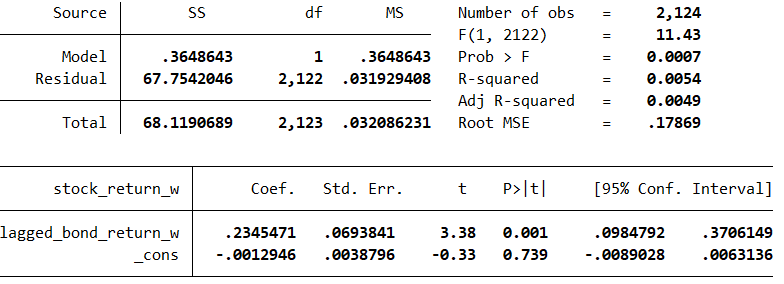
\includegraphics[trim={0 0 0 0},clip,width=1.0\linewidth]{figures/regression-results/regression-high-yield-ccc-d-moodies-stocks-as-dependent.PNG}
	\caption{Results: regression with high-yield corporate bonds (as by Moody's) as independent variable, and stocks as dependent variable}
	\label{fig:regression-high-yield-ccc-d-moodies-stocks-as-dependent.PNG}
\end{figure}







%TODO ratings generation

